%%%%%%%%%%%%%%%%%%%%%%%%%%%%%%%%%%%%%%%%%
%% Data section
\section{Data and Institutional Context}
\label{sec:data}

\subsection{Data Description}
The data used in this analysis come from two primary sources: \citet[IPEDS]{ipeds} regarding institutional information on finances and enrolment, and \citet[IBHED]{ibhed} for data on every professor in the Illinois public university system.

IPEDS is a survey of higher educational institutions in the US, and legally requires institutions to participate in order to receive Federal Title IV student aid.\footnote{
    This statement means that IPEDS does not necessarily cover the universe of US higher education institutions, yet in practice every public university and not for-profit four-year institution is represented.
}
Data are consistent between the years 1990 and 2021,\footnote{
    The years 1987-1989 are represented in these data in an incompletion fashion, so I focus on the years 1990 onwards.
    Year refers to the calendar year of the spring term --- i.e. 1987 refers to the academic year that ran August 1986 to July 1987.
}
and provide information on the total revenues a university received from every source (including state governments), enrolment number, plus faculty count and total expenditures on salaries.\footnote{
    I combine the Urban Institute's 2018 compilation of IPEDS data for the years 1990-2017, and manually combine with raw NCES data regarding the year 2018-2021 for all relevant variables.
    Figures for enrolment, faculty counts and salaries come from the raw NCES version of IPEDS for all years to address inconsistencies in the Urban Institute's data formulation for these variables.
}
I restrict analysis to public, four-year, degree-granting institutions, as these institutions adhere to a standardised concept of faculty profile, where tenure and title of appointment (lecturer, assistant professor, etc.) are relatively standardised.
For-profit institutions employ and enrol a negligible share of professors and students respectively, while students at two-year institutions by majority intend to eventually enrol at a four-year institution \citep{mountjoy2022},\footnote{
    Furthermore, \cite{mountjoy2022} documents the effects of expanding two-year higher education access in the US separately for students who would have and those who would not have otherwise have attended college.
    The high rate of eventual enrolment at four-year institutions among two-year students explains the negative impact of increased access to two-year institutions on students who are diverted away from four-year institutions.
}
so that these institutions are not considered.

IPEDS reports the count of professors employed by position, as well as total salary expenditures by position.
This gives a resulting panel data-set, where each row represents a university-year, and includes columns for university finances, plus total count and average salary\footnote{
    Real salary is computed by scaling nominal salary to 2021 dollars by the CPI-U.
} for professors by position (lecturer, assistant, tenured, total).
\autoref{tab:ipeds-summary} presents summary statistics for relevant variables in these data.

\begin{table}[h!]
    \singlespacing
    \centering
    \caption{IPEDS Summary Statistics, Public Universities Panel 1987--2021}
    \makebox[\textwidth][c]{
\begin{tabular}{@{\extracolsep{5pt}}lcccc} 
\\[-1.8ex]\hline 
\hline \\[-1.8ex] 
Statistic & \multicolumn{1}{c}{Mean} & \multicolumn{1}{c}{St. Dev.} & \multicolumn{1}{c}{Median} & \multicolumn{1}{c}{N} \\ 
\hline \\[-1.8ex] 
Enrollment, full-time equivalent & 11,511 & 10,821 & 7,723 & 18,504 \\ 
State appropriations (millions 2021 USD) & 99 & 125 & 52 & 18,504 \\ 
Total revenues (millions 2021 USD) & 425 & 793 & 158 & 18,504 \\ 
Lecturers count & 60 & 74 & 34 & 17,329 \\ 
Assistant professors count & 113 & 102 & 84 & 17,826 \\ 
Full professors count & 261 & 284 & 162 & 17,929 \\ 
All professors count & 429 & 437 & 284 & 18,504 \\ 
Lecturers mean salary (2021 USD) & 58,212 & 13,244 & 56,215 & 16,686 \\ 
Assistant mean salary (2021 USD) & 74,319 & 13,849 & 72,191 & 17,750 \\ 
Full mean salary (2021 USD) & 99,675 & 23,590 & 95,229 & 17,837 \\ 
All mean salary (2021 USD) & 81,570 & 25,055 & 80,582 & 17,759 \\ 
\hline \\[-1.8ex] 
\end{tabular} 
}
    \label{tab:ipeds-summary}
\end{table}

IPEDS provides information at the university level, yet lacks information on the distribution of salaries and professor count within a university.\footnote{
    IPEDS provides total paid to salary and total faculty employed per university-year, so that I can investigate average professor salary per university-year with IPEDS data.
    Unfortunately, this measure of professors' salaries is particularly crude in measuring on professors' salaries and other individual-outcomes; summary statistics on IPEDS data do not agree with trends in average professor salary over the sample time period \citep{aau2021survey}.
    Similarly, IPEDS reports of the average salary paid to professors at private institutions also disagree with other sources, so are not considered in this analysis.
}
To investigate the distribution, I integrate individual-level data for every public university professor in the state of Illinois between the years 2010-2021.
IBHED hosts the information;
Public Act 96-0266 (effective 1 January 2010) requires that each university report base salary and benefits all administrators, faculty members, and instructors employed by the college or university.\footnote{
    The universities included are all campuses of the nine Illinois public universities: Chicago State University, Eastern Illinois University, Governors State University, Illinois State University, Northeastern Illinois University, Northern Illinois University, Southern Illinois University  (all five campuses), University of Illinois (all four campuses), Western Illinois University.
}
This publicly available data provides the basis to build a panel of Illinois public university professors 2010-2021; I define a professor as an individual by their first plus last name and university pairing, and link this database to IPEDS regarding finances for their employing institution.

The analysis sample represents 16,932 professors in the year 2010 and 15,352 in the year 2021, with summary statistics presented in \autoref{tab:illinois-summary}.
Additionally, further analysis using the first year of a professor's employment focuses on the subset of professors with observed year of hiring between the years 2011 and 2021, representing 1,778 professors in 2011, and 9,099 in 2021.\footnote{
    Summary statistics for this group, which over-represents lecturers compared to assistant and full professors, can be seen in \autoref{tab:illinois-summary-rolling}.
    The reasons for considering the sub-sample with identified year of hire in the range 2011-2021 are explained in \autoref{sec:iv-model-indiv}.
}

\begin{table}[h!]
    \singlespacing
    \centering
    \caption{IBHED Summary Statistics, Professor Panel 2010--2021.}
    \makebox[\textwidth][c]{
\begin{tabular}{@{\extracolsep{5pt}}lcccc} 
\\[-1.8ex]\hline 
\hline \\[-1.8ex] 
Statistic & \multicolumn{1}{c}{Mean} & \multicolumn{1}{c}{St. Dev.} & \multicolumn{1}{c}{Median} & \multicolumn{1}{c}{N} \\ 
\hline \\[-1.8ex] 
Lecturer, percent & 39 & 49 & 0 & 60,926 \\ 
Assistant professor, percent & 33 & 47 & 0 & 60,926 \\ 
Full professor, percent & 12 & 32 & 0 & 60,926 \\ 
Administrator professor, percent & 17 & 37 & 0 & 60,926 \\ 
Lecturer salary (2021 USD) & 27,280 & 25,579 & 17,738 & 23,618 \\ 
Assistant salary (2021 USD) & 79,352 & 37,038 & 75,339 & 19,865 \\ 
Full salary (2021 USD) & 108,411 & 58,988 & 97,978 & 7,228 \\ 
Administrator salary (2021 USD) & 110,020 & 62,547 & 98,258 & 10,215 \\ 
All salary (2021 USD) & 67,755 & 54,259 & 64,750 & 60,926 \\ 
Lecturer benefits (2021 USD) & 1,944 & 7,190 & 0 & 23,618 \\ 
Assistant benefits (2021 USD) & 2,886 & 7,228 & 0 & 19,865 \\ 
Full benefits (2021 USD) & 5,937 & 13,734 & 0 & 7,228 \\ 
Administrator benefits (2021 USD) & 3,129 & 19,465 & 0 & 10,215 \\ 
All benefits (2021 USD) & 2,924 & 11,155 & 0 & 60,926 \\ 
\hline \\[-1.8ex] 
\end{tabular} 
}
    \label{tab:illinois-summary}
\end{table}

\subsection{Trends in Finances, Enrolment, and Faculty Composition}
\label{sec:trends}
A state government plans an annual budget a couple of years ahead of the fiscal year, and the legislature chooses to approve or reject a budget request put forth by the governor's office.\footnote{
    \cite{NBERw23736} present a full discussion of the decision-making process for state appropriations, drawing on administrative records originally analysed by \cite{parmley2009state}.
}
US state governments, by majority, are legally obligated to run a balanced-budget, so that yearly variation in tax revenues (caused by changing economic conditions or otherwise) necessarily affect state expenditures.
This process leads to yearly variation in state appropriations not seen in other revenues sources (such as federal government appropriations), since US states differ in their support for higher education, and are subject to fiscal constraints.
State appropriations to higher education are a particularly attractive area of state spending to absorb such shocks to state finances \citep{delaney2011state}.\footnote{
    \cite{delaney2011state} fully describes the financial environment of state expenditures, and what makes spending on higher education an attractive area for state governments to expand funding during years of higher tax revenues, and retract funding in leaner years.
    An analysis of state expenditures for the years 1980-2004 (overlapping with the sample for this analysis) provides solid evidence for these trends.
}
Additionally, there is yearly variation in the number of higher education students in each state \citep{turner2014impact}, so that per-student state appropriations vary on multiple dimensions.

\autoref{fig:funding} exhibits the trends for the mean public university for the years 1990-2021.
We see a rise in total revenues received by public universities (from all sources), and a notable increase in mean tuition revenues from \$48 million per year-university to \$150 million per year-university.
At the same time, total state appropriations stagnated at around \$100 million per year-university for 1990-2008, falling around 2008 and have not recovered ever since.
While public universities experienced a stagnation in state support, private universities were not exposed to the same constraints, receiving \$37,000 per student in 1990 and \$49,000 in 2021, experiencing no corresponding decline in any specific component.

\begin{figure}[h!]
    \centering
    \singlespacing
    \caption{Mean Total Revenues among Public Universities, by Year.}
    \begin{subfigure}[b]{0.495\textwidth}
        \centering
        \caption{Total, millions \$ 2021 CPI-U.}
        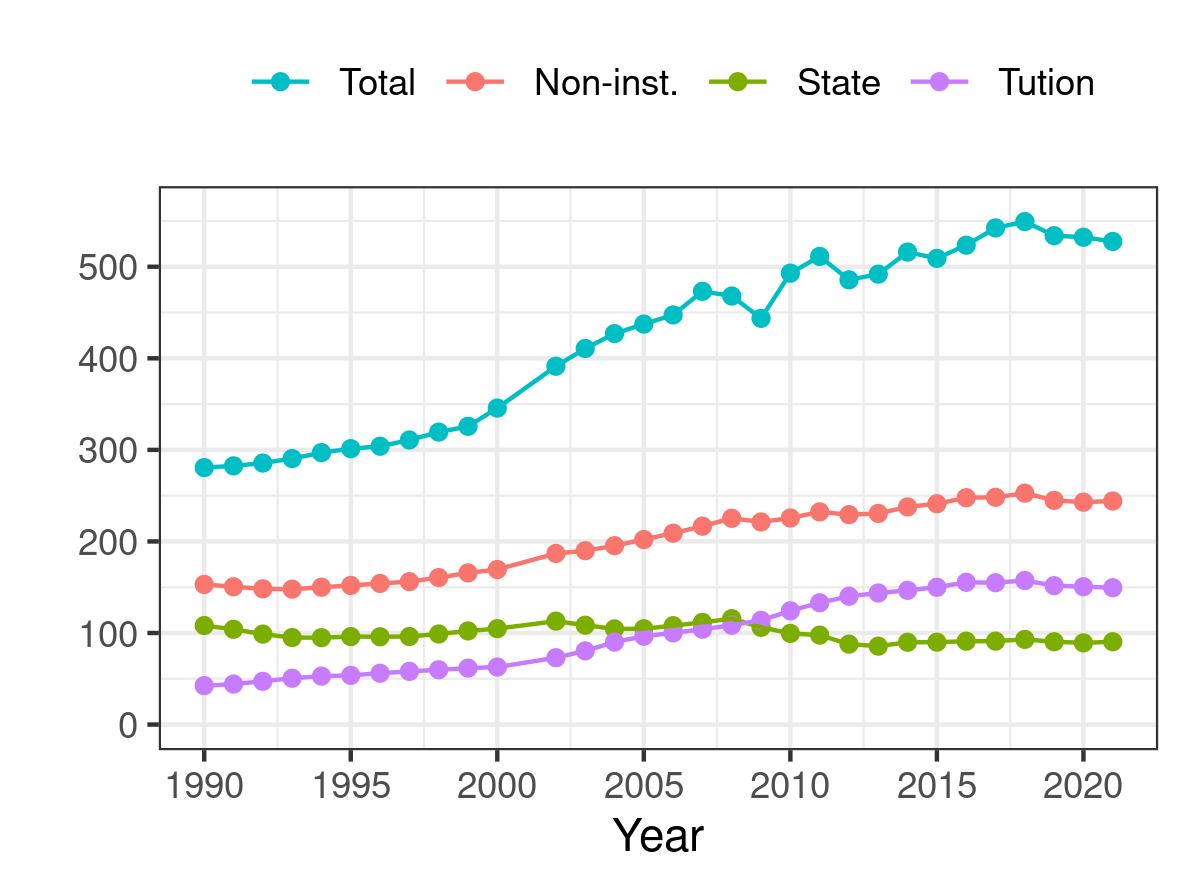
\includegraphics[width=\textwidth]{figures/mean-funding-total.png}
        \label{fig:mean-funding-total}
    \end{subfigure}
    \begin{subfigure}[b]{0.495\textwidth}
        \centering
        \caption{Per Enrolled Student, \$ 2021 CPI-U.}
        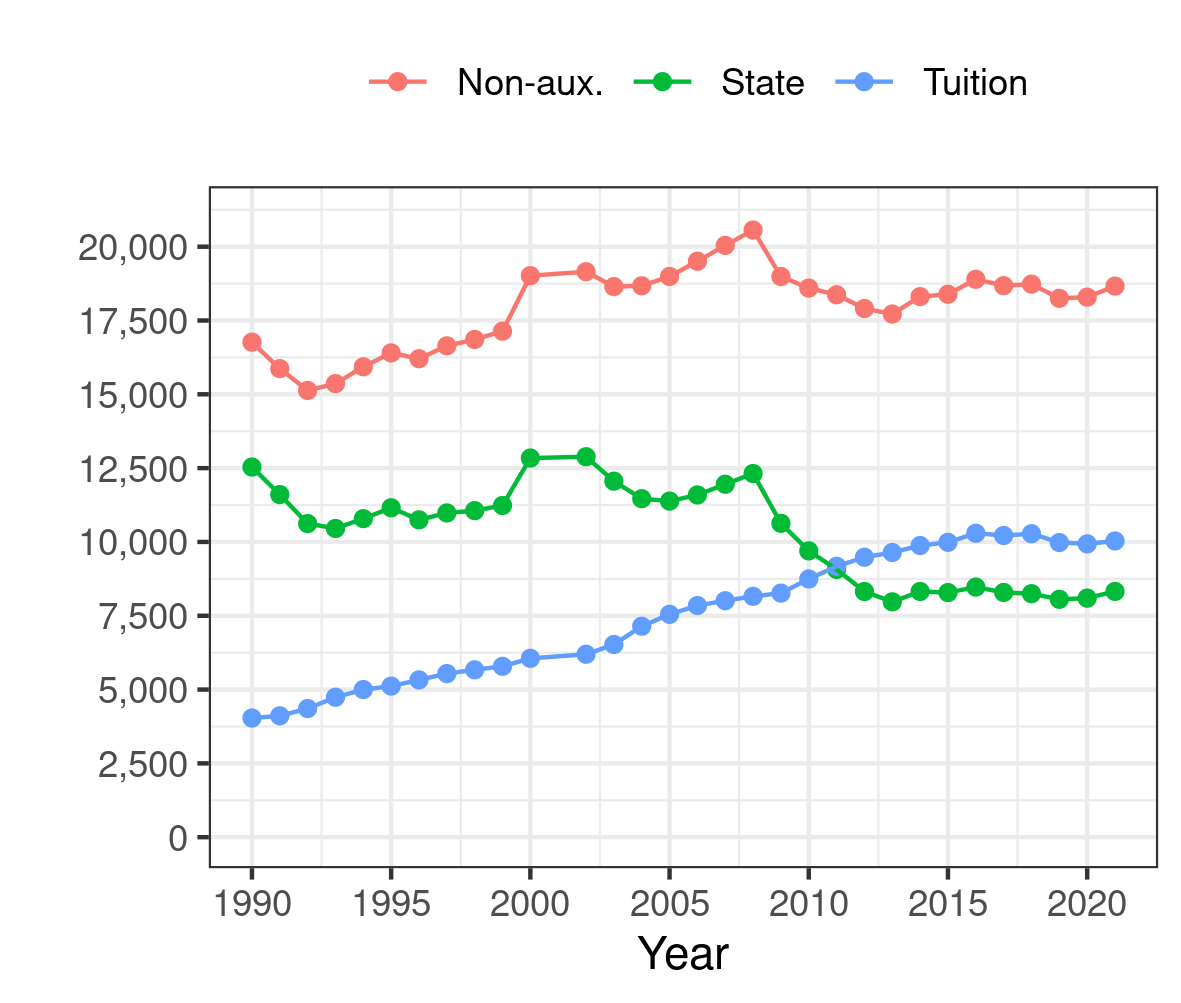
\includegraphics[width=\textwidth]{figures/mean-funding-fte.png}
        \label{fig:mean-funding-fte}
    \end{subfigure}
    \label{fig:funding}
\end{figure}

\begin{figure}[h!]
    \centering
    \singlespacing
    \caption{Total Student enrolment, by University Sector, and Year.}
    \begin{subfigure}[b]{0.495\textwidth}
        \centering
        \caption{Total.}
        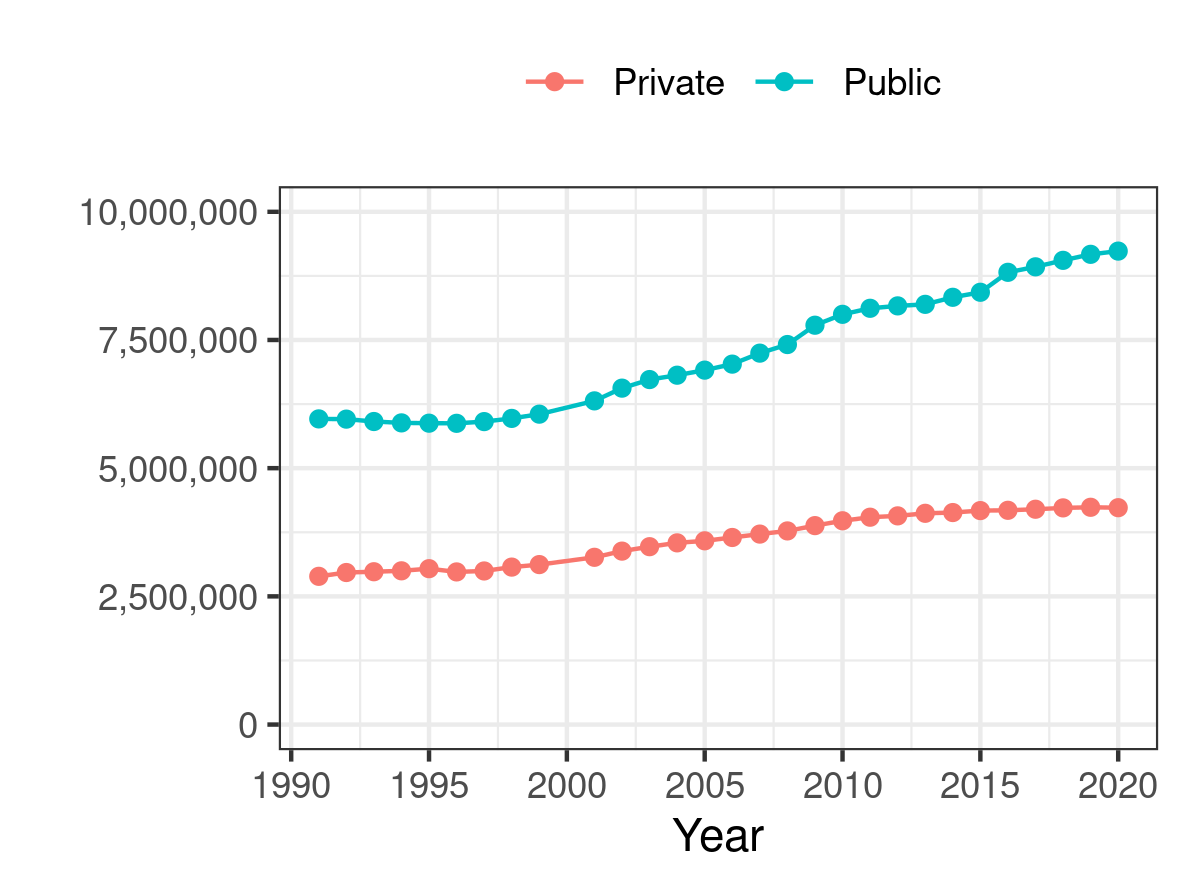
\includegraphics[width=\textwidth]{figures/enrollment-total.png}
        \label{fig:enrollment-total}
    \end{subfigure}
    \begin{subfigure}[b]{0.495\textwidth}
        \centering
        \caption{Mean, University Level.}
        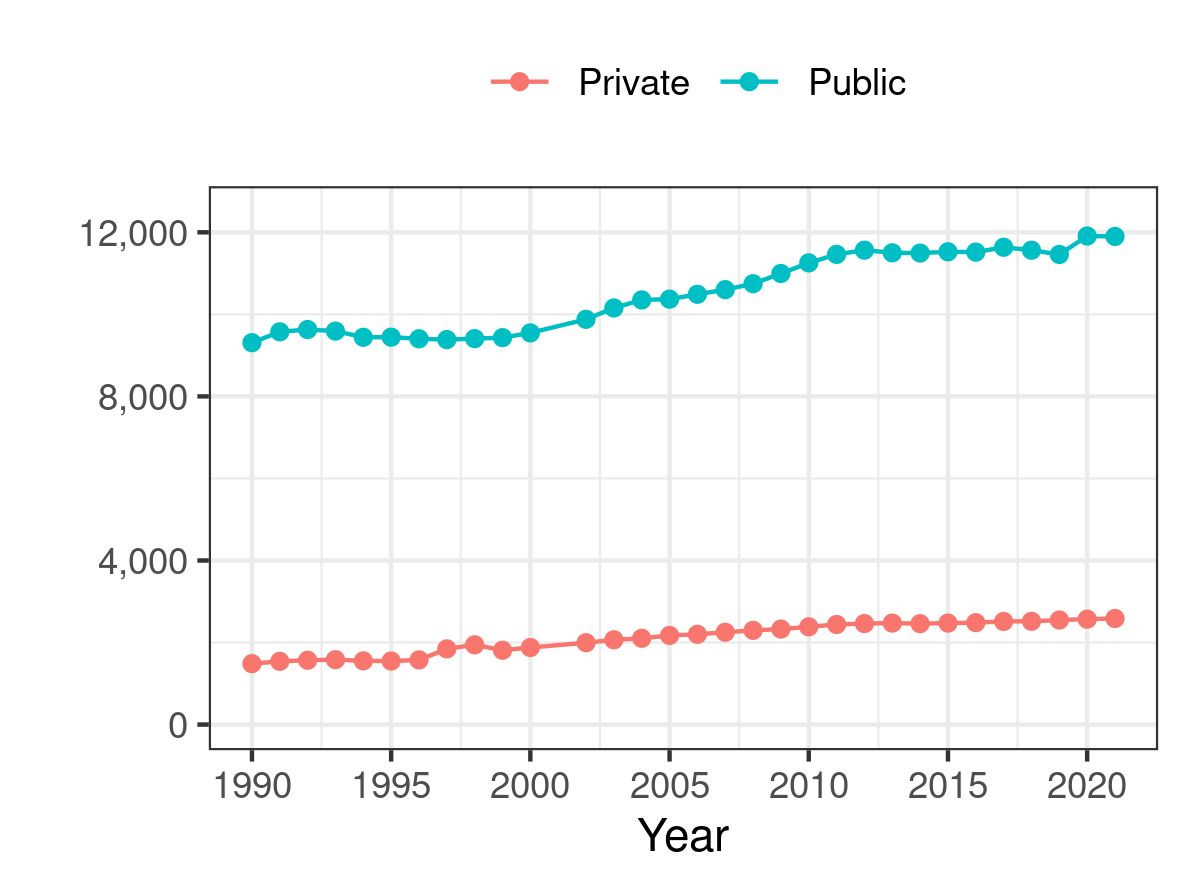
\includegraphics[width=\textwidth]{figures/enrollment-mean.png}
        \label{fig:enrollment-mean}
    \end{subfigure}
    \label{fig:enrolment}
\end{figure}

At the same time, student enrolment at public universities rose precipitously.
6.2 million students were enrolled in public universities in 1990, and this number rose by 47\% to 9.1 million, with most of the increase occurring over the years 2000-2021.
\autoref{fig:enrolment} shows that total enrolment at private universities has also risen over the same time period, but not as drastic in either relative or absolute terms; the mean private university grew from 9,800 students in 1990 to 11,800 in 2021.
This means that revenues per student have stagnated across all measures (seen in \autoref{fig:mean-funding-fte}), and particularly fallen from a mean of \$11,000 per student in 1990 to less than \$8,000 per student in 2021.

\begin{figure}[h!]
    \centering
    \singlespacing
    \caption{Student Enrollment per Professor, by University Sector, Professor Appointment, and Year.}
    \begin{subfigure}[b]{0.495\textwidth}
        \centering
        \caption{Lecturer}
        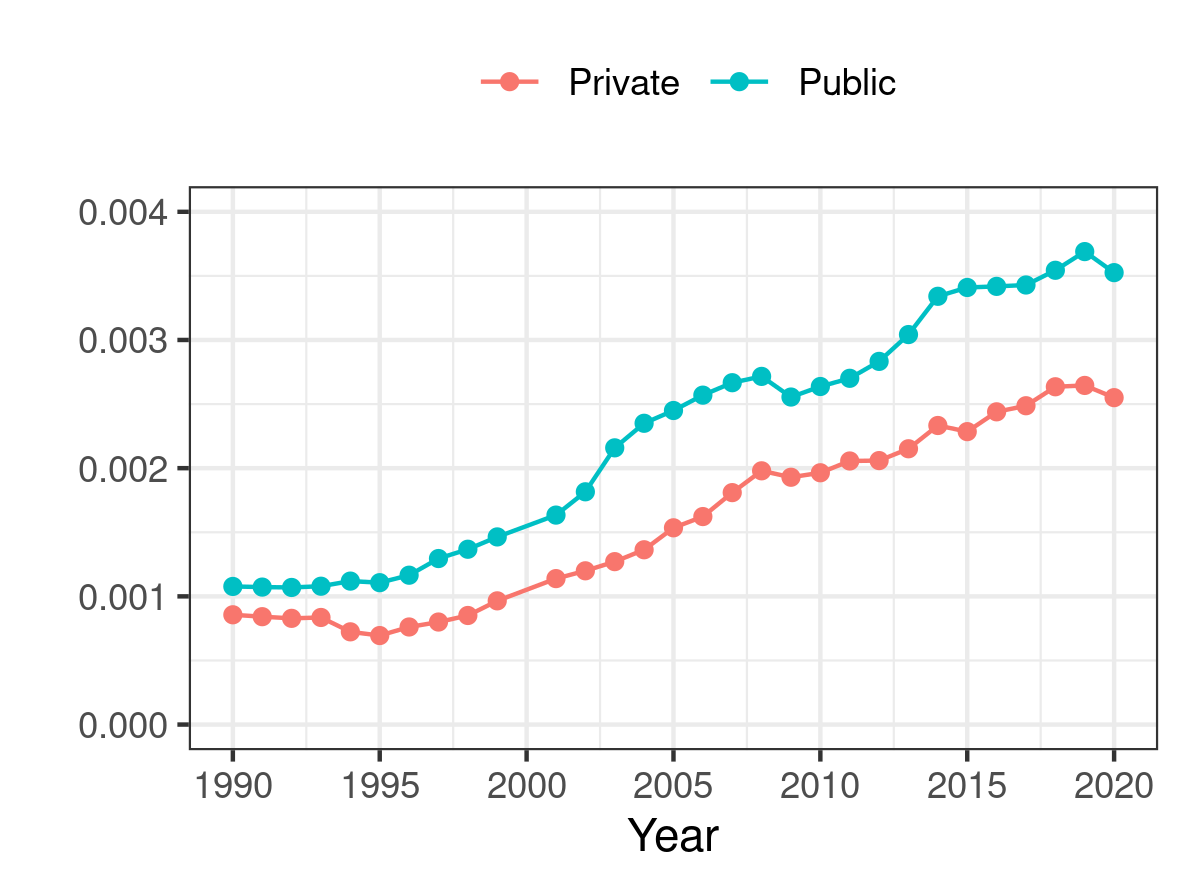
\includegraphics[width=\textwidth]{figures/lecturer-fte-perprof.png}
        \label{fig:lecturer-fte-perprof}
    \end{subfigure}
    \begin{subfigure}[b]{0.495\textwidth}
        \centering
        \caption{Assistant.}
        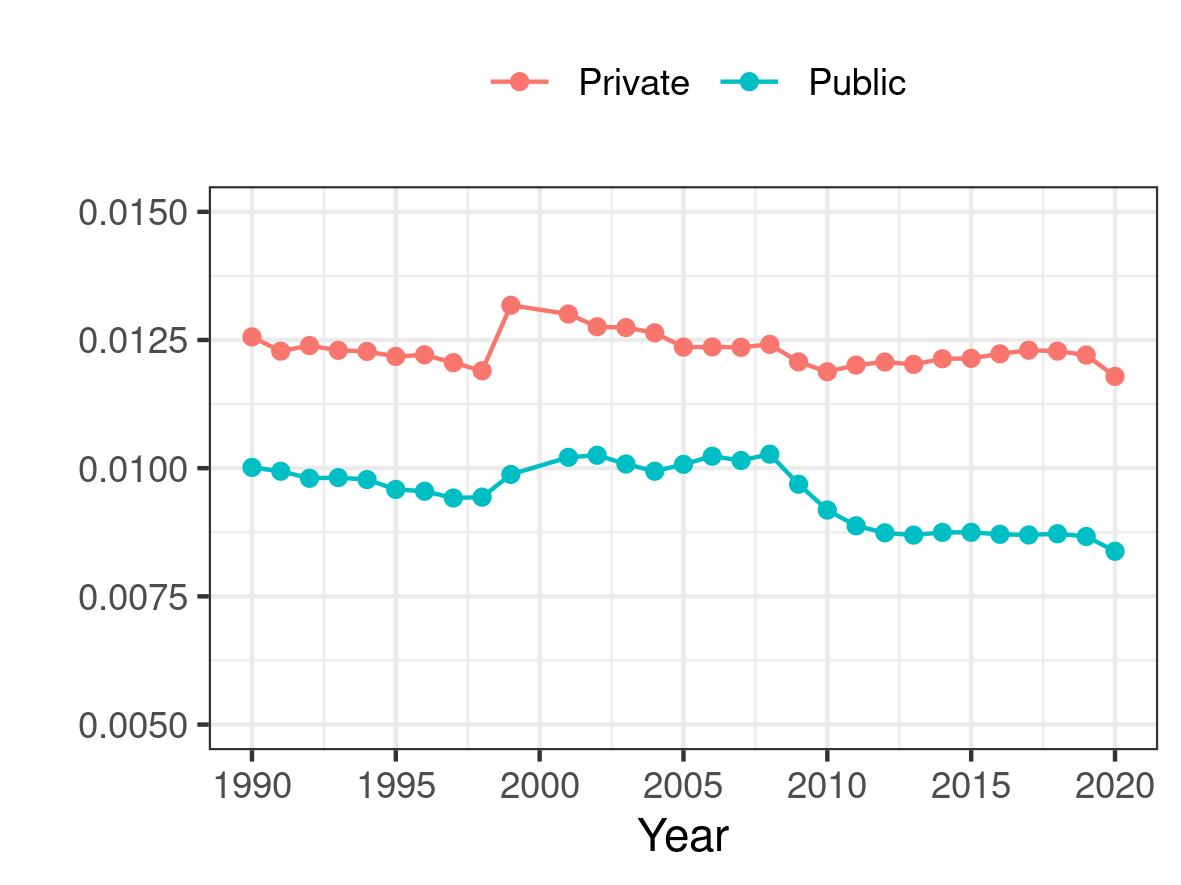
\includegraphics[width=\textwidth]{figures/assistant-fte-perprof.png}
        \label{fig:assistant-fte-perprof}
    \end{subfigure}
    \begin{subfigure}[b]{0.495\textwidth}
        \centering
        \caption{Full.}
        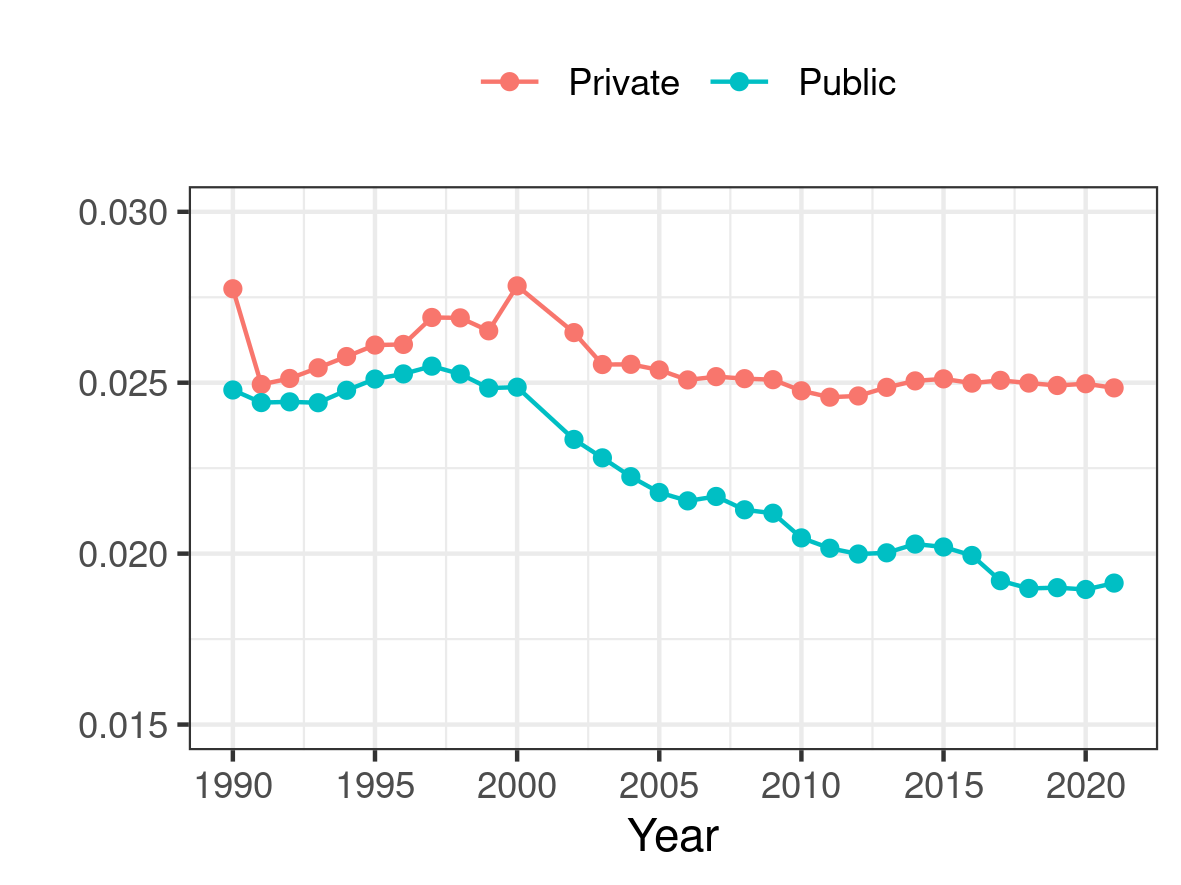
\includegraphics[width=\textwidth]{figures/full-fte-perprof.png}
        \label{fig:full-fte-perprof}
    \end{subfigure}
    \begin{subfigure}[b]{0.495\textwidth}
        \centering
        \caption{All.}
        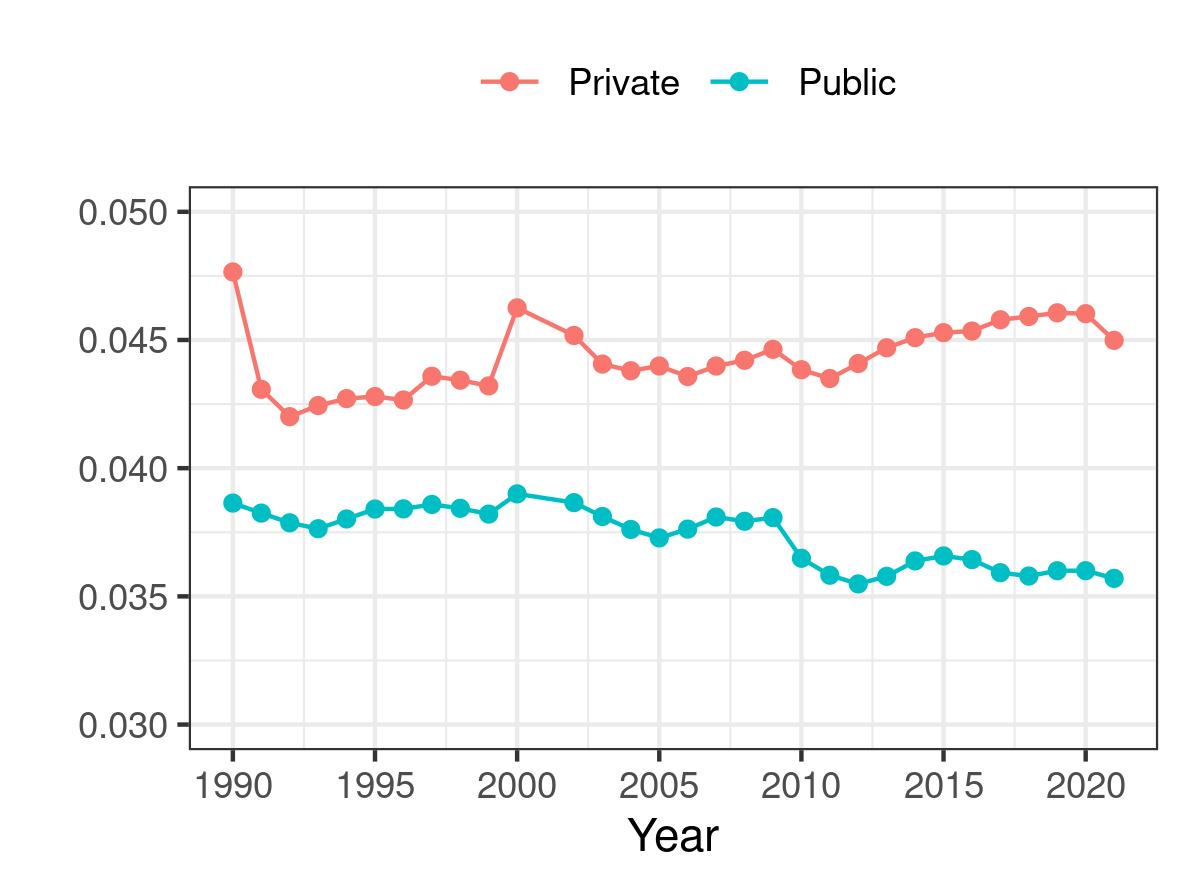
\includegraphics[width=\textwidth]{figures/all-fte-perprof.png}
        \label{fig:all-fte-perprof}
    \end{subfigure}
    \label{fig:fte-perprof}
\end{figure}

\autoref{fig:fte-perprof} documents the divergence in faculty composition (per student) between the average private and public university 1990-2021.
Private universities start with  a higher baseline of around 4.5 professors per 100 students, and exhibited yearly variation of less than 0.5 professor per hundred students over the thirty years.
Public universities start with 3.9 professors per hundred students, and this number falls to around 3.5 primarily in the 2008-2011 time period.
We see a similar difference in baseline, and fall for the years 2008-2011 for assistant professors.
Private and public universities have similar numbers of associated and full professors before the year 2000, yet this number has fallen by over 20\% in the next 20 years only for public universities: in 2021 the mean public university has 6 fewer full professors per hundred students than the mean private university.
Over the same time period, we see the rise in use of non-tenure track instructor positions (referred to as lecturers from here on), who were employed at similar rates in both sectors in 1990 yet have been utilised by public universities at a higher rate since.

\subsection{Trends in Illinois}
\label{sec:trends-illinois}

The state of Illinois experienced the same stagnation in state support for higher education that the rest of the nation has experienced 1990-2021.
\autoref{fig:illinois-funding} shows the trends for revenues among the seven Illinois public university campuses, including the falling share of state appropriations and substitution towards tuition revenue.

\begin{figure}[h!]
    \centering
    \singlespacing
    \caption{Mean Revenues among Illinois Public Universities, by Year.}
    \begin{subfigure}[b]{0.495\textwidth}
        \centering
        \caption{Total, millions \$ 2021 CPI-U.}
        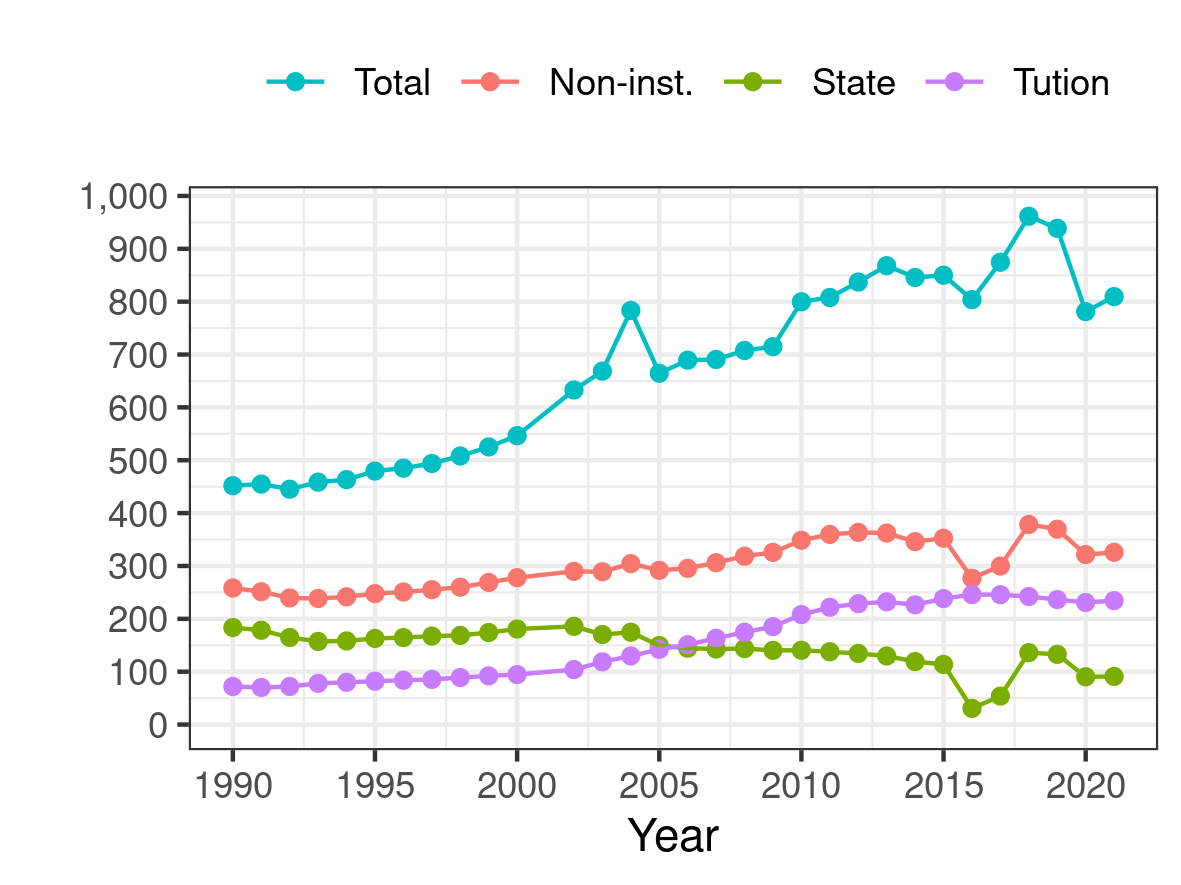
\includegraphics[width=\textwidth]{figures/illinois-funding-total.png}
        \label{fig:illinois-funding-total}
    \end{subfigure}
    \begin{subfigure}[b]{0.495\textwidth}
        \centering
        \caption{Per Enrolled Student, \$ 2021 CPI-U.}
        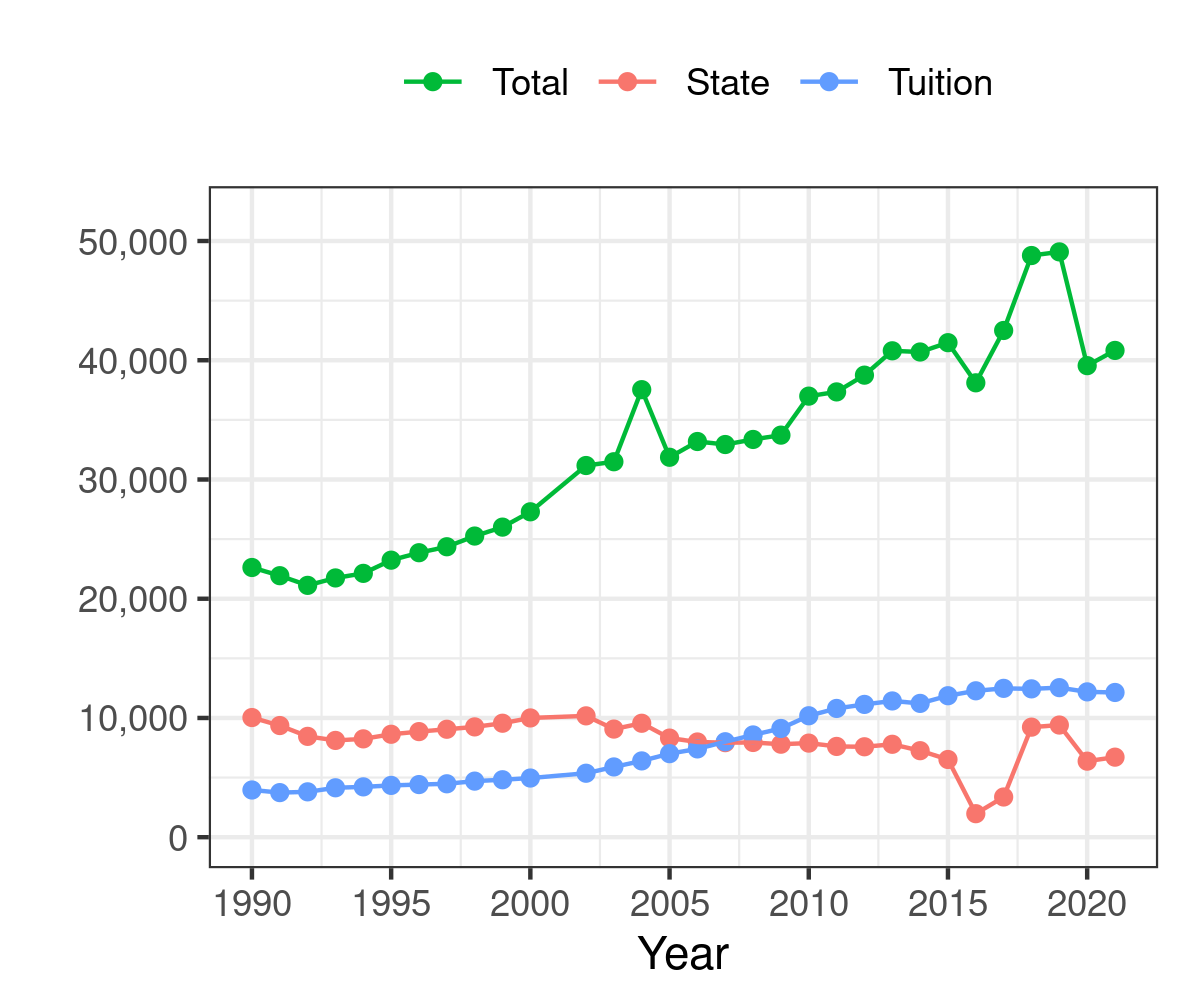
\includegraphics[width=\textwidth]{figures/illinois-funding-fte.png}
        \label{fig:illinois-funding-fte}
    \end{subfigure}
    \label{fig:illinois-funding}
\end{figure}

The decade of 2010-2021 has also seen yearly variation in its revenues, particularly around 2016.
In the calendar year 2015 partisan disagreements between the democratic legislature and republican governor led to the 2016 fiscal year starting with no state budget.
State agencies, and higher education institutions, employed accounting techniques to continue operating without any resources provided by the state government.\footnote{
    Fiscal year 2016 refers to June 205 to June 2016, as is the same for the academic year definition in this analysis. 
    K-12 schools were unaffected thanks to a separate budget agreement allowing non-higher education to operate as before.
}
While state institutions were able to stay open, there were drastic revenue and spending cuts in response to the budget impasse, as it continued through fiscal year 2017, and ended with a new budget restoring revenues to state agencies and universities for the 2018 fiscal year.
This variation in public university revenues via the state appropriations channel, stemming entirely from political disagreements --- not from state decisions regarding higher education and its finances \citep{young2020squandered} --- mean that Illinois public universities exhibit sizable changes in their state appropriations over 2010-2021, of similar order to those for the rest of the country over 1990-2021.
